\section{Cross-Domain Instantiation: Slime Mold and Transformer}


\subsection{Overview}


\S{}3 では知性的動態の三公理を提示し、\S{}4 ではそれを記述するための IFGT 語彙と Tero-Kobayashi-Nakagaki モデルとの語彙対応を示した。これらはいずれも構造論的記述であり、特定の substrate を前提しない。

本セクションは、この \textbf{substrate 非依存性} を構造的に検査する。具体的には、生物物理学的に最もよく研究されている動的系の一つである粘菌(\emph{Physarum polycephalum})と、現代の人工知能アーキテクチャの中核である Transformer という、\textbf{substrate・スケール・実装} において根本的に異なる二系を取り上げる。両者を \S{}3 の三公理と \S{}4 の IFGT 語彙のもとに構造的に対応するものとして記述することで、本論文の枠組みが領域横断的に適用可能であることを検討する。

ここで重要な但し書きを冒頭で明示する。本セクションは粘菌と Transformer の \textbf{構造的同型性} のみを主張し、両者の \textbf{意味論的・経験的・認知的同一性} は一切主張しない。粘菌が「考える」、Transformer が「理解する」── これらの問いは本論文の射程外であり、構造的同型性とは独立の問題である。両者の混同(構造同型から認知同一性への飛躍)が、知性論を繰り返し混乱させてきた典型的誤謬であり、本セクションはこの誤謬を明示的に避ける。

\subsection{The slime mold as an externally validated instantiation}


\subsubsection{Independent biological grounding}


粘菌の管網動態は、本論文の枠組みからは独立に、生物物理学的に既に詳細に研究されている。これは本論文の三公理が \textbf{独自構成ではない} ことを示す外部的な支持例として読みうる。

研究系列の主要な節目を簡潔に挙げる:

\begin{itemize}
\item \textbf{Nakagaki et al. (2000)} \citep{Nakagaki2000}:粘菌が迷路の二点間で \textbf{最短経路} を実現する現象を、知性概念に依拠せず純粋に生物物理学的観察として報告した
\item \textbf{Kobayashi, Tero \& Nakagaki (2006)} \citep{Kobayashi2006}:粘菌のリズム的原形質運動の数理モデルを構築した。本論文の第二公理(時間順序付け)に対応する具体実例
\item \textbf{Tero, Kobayashi \& Nakagaki (2007)} \citep{Tero2007}:flow-reinforcement と decay の最小動力学方程式系として Physarum solver を定式化した(\S{}4.4.1 に詳述)
\end{itemize}

これらの研究系列は、共通して \textbf{「smart behavior は能力ではなく動力学である」} という構造論的立場を取っている。中垣自身の表現「粘菌は知能を持たないが、知能的に振る舞う」は、本論文の中心立場 ── 知性は能力でも所有物でもなく、構造的条件下で成立する力学的状態である(\S{}1.2, \S{}3.6) ── と、\textbf{まったく異なる研究路線から同じ場所に到達している}。

\subsubsection{Mapping to the three axioms}


粘菌動態を \S{}3 の三公理のもとに整理する。モデル方程式の詳細は \S{}4.4 を参照。

\textbf{第一公理(連結状態空間):}
粘菌の管網ネットワーク $\{N_i, e_{ij}\}$ は、状態空間の連結構造そのものとして機能する。ノード(接続点)は栄養源・分岐点として、エッジ(管)は物質と信号の伝播経路として、グラフ構造を構成する。粘菌は初期段階で迷路全体を充填するように管網を展開し、これによって連結性が保証される。連結性は単なる空間的隣接ではなく、Kirchhoff 則による流量保存が成立する \textbf{動的連結性} である。

\textbf{第二公理(時間順序付け):}
管の伝導度 $D_{ij}$ は時間発展方程式

\[
\frac{dD_{ij}}{dt} = f(|Q_{ij}|) - D_{ij}
\]

に従って進化する(\S{}4.4.1)。これは抽象的には $s_{t+1} = F_\text{bio}(s_t)$ と書ける状態更新であり、外部時計を要求しない。重要なのは、強化(reinforcement)と減衰(decay)の競合が \textbf{過去の流量履歴を現在の伝導度に累積させる} 点である。この履歴依存性が、第二公理の意味での時間的順序付けを構成する。

\textbf{第三公理(グローバル制約 $\Phi_\text{bio}$):}
粘菌動態における大域バイアスは、\textbf{栄養源を頂点とする境界条件} と \textbf{Kirchhoff 則による流量保存} の組み合わせから生じる。これは形式的には

\[
\Phi_\text{bio} : \mathcal{S} \to \mathbb{R}
\]

として表現されるスカラー場である。$\Phi_\text{bio}$ は栄養源勾配・エネルギーコスト・物理的境界条件を統合した大域的制約であり、\S{}3.3 で要請した \textbf{局所更新規則の単純集約への非還元性} を満たす。局所的に well-defined な flow-reinforcement だけでは shortest path は現れない ── 大域条件が局所動態を制約することで、初めて大域構造が動的に創発する(\S{}4.4.3 を参照)。

\subsubsection{The structural status of the slime mold case}


粘菌の構造論的地位を明示する:

\begin{itemize}
\item 粘菌動態は \S{}3 の三公理を満たす具体例として読める
\item 粘菌の動態は \S{}4 の IFGT 語彙によって粗視化・投影的に記述できる
\item 粘菌に関する独立な実証研究(Nakagaki, Tero, Kobayashi ら)は、本論文の構造論的議論と \textbf{独立に収束している}
\item これは本論文の枠組みが「独自構成」ではなく「複数の研究路線が到達しうる構造」であることを示唆する
\end{itemize}

\subsection{The transformer as an artificial instantiation}


\subsubsection{Why the transformer}


Transformer アーキテクチャ \citep{Vaswani2017} は、現代の人工知能における代表的な動的系である。本セクションが Transformer を選ぶのは、その認知科学的解釈や工学的成功のためではなく、以下の構造的理由による:

\begin{itemize}
\item Transformer は \textbf{生物的 substrate を持たない} ── 粘菌との対比として、substrate 非依存性の最も鋭い例となる
\item Transformer は \textbf{層別の明示的構造} を持つ ── 三公理との対応が形式的に追跡可能である
\item Transformer は \textbf{既に十分に研究されている} ── 構造記述に学術的合意がある
\item Transformer の動態は \textbf{大規模に観測されている} ── 構造的記述の検証が経験的に可能である
\end{itemize}

これらの理由から、Transformer は粘菌との cross-domain 比較対象として、最も鋭い選択である。

\subsubsection{Mapping to the three axioms}


Transformer の動態を \S{}3 の三公理のもとに整理する。

\textbf{第一公理(連結状態空間):}
トークン列を入力とする Transformer において、状態空間は層別隠れベクトルの集合

\[
\mathcal{S} = \{ h^{(\ell)}_i \}
\]

として表現される(ここで $\ell$ は層、$i$ はトークン位置)。連結性は \textbf{attention 機構} によって与えられる:任意のトークン位置 $i$ の表現は、attention を通じて他の任意の位置 $j$ と関係的に接続される。これにより状態空間は実質的に連結された関係空間を形成する。連結性は粘菌の場合のような物理的接続ではなく、\textbf{計算上の関係的接続} であるが、\S{}3.1 で要請された連結性の構造的条件(状態間の到達可能性)は満たされる。

\textbf{第二公理(時間順序付け):}
Transformer は層別の状態更新を行う:

\[
h^{(\ell+1)} = F_\text{tr}\!\left( h^{(\ell)} \right)
\]

ここで $F_\text{tr}$ は attention と feed-forward 操作からなる層変換である。層順序は \textbf{時間的順序の最小の意味} ── 更新が同時に起こらず、変化が累積する ── を満たす。これは物理的時間ではなく \textbf{計算的時間} であるが、\S{}3.2 で要請された構造的条件(同時更新の否定と変化の累積)を満たす。

\textbf{第三公理(グローバル制約 $\Phi_\text{tr}$):}
Transformer の動態に大域バイアスを与えるのは、訓練時の \textbf{損失関数} である:

\[
\Phi_\text{tr} : \mathcal{S} \to \mathbb{R}
\]

として表現されるこの大域制約は、訓練時には勾配降下を通じて表象動態全体に作用し、推論時にはその結果として学習されたパラメータ構造を通じて間接的に作用する。$\Phi_\text{tr}$ は意味でも目的でもなく、訓練データ分布から誘導される \textbf{構造的バイアス} である。重要なのは、$\Phi_\text{tr}$ も粘菌の $\Phi_\text{bio}$ と同様に、\textbf{局所更新規則の単純集約には還元されない} という点である。個々の attention 計算からは大域的表象構造は導出されない ── 訓練を通じた大域的整合化が、局所動態を制約することで初めて意味のある表象動態が形成される。

\subsubsection{What this mapping does not assert}


Transformer の \S{}3 三公理への対応は、以下を \textbf{主張しない}:

\begin{itemize}
\item Transformer が「理解する」(understand) ── \S{}3 公理は意味論を導入しない
\item Transformer が意識を持つ ── 意識は本論文の射程外
\item Transformer の動態が認知的に妥当である ── 構造的同型性は認知的妥当性を含意しない
\item Transformer が「真の」知性である ── 「真の」という限定子は規範的概念であり、構造論には現れない
\end{itemize}

本論文が主張するのは唯一、Transformer が \S{}3 の三公理を \textbf{構造的に満たす} という点のみである。

\subsection{Structural homology and its limits}


\subsubsection{What the homology asserts}


粘菌と Transformer の構造的対応を以下に整理する:

\begin{table}[H]
\centering
\small
\begin{tabularx}{\textwidth}{>{\raggedright\arraybackslash}X>{\raggedright\arraybackslash}X>{\raggedright\arraybackslash}X}
\toprule
公理 & 粘菌 & Transformer \\
\midrule
\textbf{連結状態空間} & 管網ネットワーク $\{N_i, e_{ij}\}$ & 層別隠れベクトル空間 $\{h^{(\ell)}_i\}$ \\
\textbf{時間順序付け} & $dD_{ij}/dt = f(\lvert Q\rvert) - D_{ij}$ & $h^{(\ell+1)} = F_\text{tr}(h^{(\ell)})$ \\
\textbf{グローバル制約 $\Phi$} & $\Phi_\text{bio}$:栄養源 + Kirchhoff 則 & $\Phi_\text{tr}$:訓練時損失関数 \\
\textbf{substrate} & 生物的(原形質) & 計算的(浮動小数点演算) \\
\textbf{時間スケール} & 時間〜日 & マイクロ秒〜秒 \\
\textbf{空間スケール} & センチメートル〜メートル & 抽象的計算空間 \\
\bottomrule
\end{tabularx}
\end{table}


両者は substrate・スケール・実装において \textbf{根本的に異なる}。それにもかかわらず、\S{}3 の三公理のもとで \textbf{構造的に対応する}。これが構造的同型性の主張内容である。

\subsubsection{What the homology does not assert}


構造的同型性から以下のいずれも \textbf{導出されない}:

\begin{itemize}
\item 認知的同一性:粘菌と Transformer が「同じように考える」とは主張しない
\item 経験的同一性:両者が同じ経験的内容を持つとは主張しない
\item 機能的同一性:両者が同じタスクを同じ方法で解くとは主張しない
\item 倫理的同一性:両者が同等の倫理的地位を持つとは主張しない
\end{itemize}

これらはすべて、構造的同型性の \textbf{上位} に位置する別個の問いである。本論文はこれらの問いを否定するのでも肯定するのでもなく、本論文の射程外として明示的に \textbf{保留} する。

\subsubsection{Why the homology nonetheless matters}


ではなぜ構造的同型性のみを論じることに意味があるのか。本セクションが構造的同型性のみを論じる積極的理由は以下である:

\textbf{substrate 非依存性の確認:}
\S{}3 の三公理は意味論的に中立に定式化されたが、その substrate 非依存性は理論的にのみ主張されていた。粘菌と Transformer の同型性は、この substrate 非依存性が \textbf{経験的にも検討可能である} ことを示す。

\textbf{規範性の密輸入の回避:}
両者の同型性を構造レベルで議論することによって、「人間中心の知性概念」が両者を比較する際に密輸入されることを避けうる。粘菌が「劣った」知性で、Transformer が「真の」知性に近づきつつある ── このような比較はいずれも公理レベルでは成立しない。

\textbf{後続セクションへの基盤:}
\S{}7(正しさの不安定化)、\S{}8(個体内非閉)、\S{}9(differential horizon)で示される構造的帰結は、\S{}3 の三公理に立脚する。本セクションが二系で同型性を示すことで、これら後続セクションの議論を \textbf{substrate を問わず検討する} ための構造的基盤が与えられる。

\subsection{The structural meaning of cross-domain convergence}


本セクションが示したのは単なる「比較」ではない。粘菌(生物物理学的研究)・Transformer(計算機科学的研究)・本論文(構造論的研究)の三者が、同じ三公理に \textbf{独立に到達している} という構造的事実である。

この収束は以下の構造を持つ:

\begin{itemize}
\item \textbf{生物物理学側}:Nakagaki, Tero, Kobayashi らが、知性概念に依拠せず純粋な動力学として粘菌動態を記述し、$\Phi$ の非還元性に相当する構造を独立に発見した
\item \textbf{計算機科学側}:Transformer アーキテクチャの開発者は、生物的知性の模倣ではなく工学的最適化として attention 機構と層構造を設計したが、結果として \S{}3 の三公理を満たす動的系を構築した
\item \textbf{本論文の側}:構造論的議論から、知性的動態の最小条件として三公理を要請した
\end{itemize}

三者の収束は偶然ではない。知性的動態が成立するためには、これら三条件のいずれかが必須であり、異なる研究路線がこの構造的制約に独立に到達せざるをえなかったと解釈できる。この収束の意味は \S{}10.2 で「the convergence of independent research lines」として再び論じられる。

\subsection{Summary}


本セクションの結論を以下に述べる:

\begin{quote}
粘菌と Transformer は、substrate・スケール・実装において根本的に異なるが、
\S{}3 の三公理のもとで構造的に対応し、\S{}4 の IFGT 語彙で投影的に記述しうる。
この構造的同型性は、本論文の枠組みの substrate 非依存性を支持する。
\end{quote}

\begin{quote}
構造的同型性は、認知的・経験的・倫理的同一性を含意しない。
これらの問いは本論文の射程外であり、明示的に保留される。
\end{quote}

\begin{quote}
粘菌(生物物理学)・Transformer(計算機科学)・本論文(構造論)の三者は、
同じ構造的制約に独立に到達している。
この収束は、本論文の構造論的議論が独自構成ではなく、
\textbf{構造的制約} を捉えていることを示唆する。
\end{quote}

後続セクションでは、本セクションの構造的基盤の上に以下の議論が展開される:

\begin{itemize}
\item \S{}6 では、構造的同型性が示す「停止構造」と「持続運動」の区別が、Gettier 問題の診断に応用される
\item \S{}7 では、両系で同様に発生する \textbf{正しさの累積による分岐爆発} の動力学的記述が展開される
\item \S{}8 では、両系で同様に欠如する \textbf{個体内停止演算子} の構造的非存在が論証される
\item \S{}9 では、両系で同様に要請される越境境界 ── \emph{the differential horizon of intelligence} ── が命名される
\end{itemize}

\begin{figure}[H]
\centering
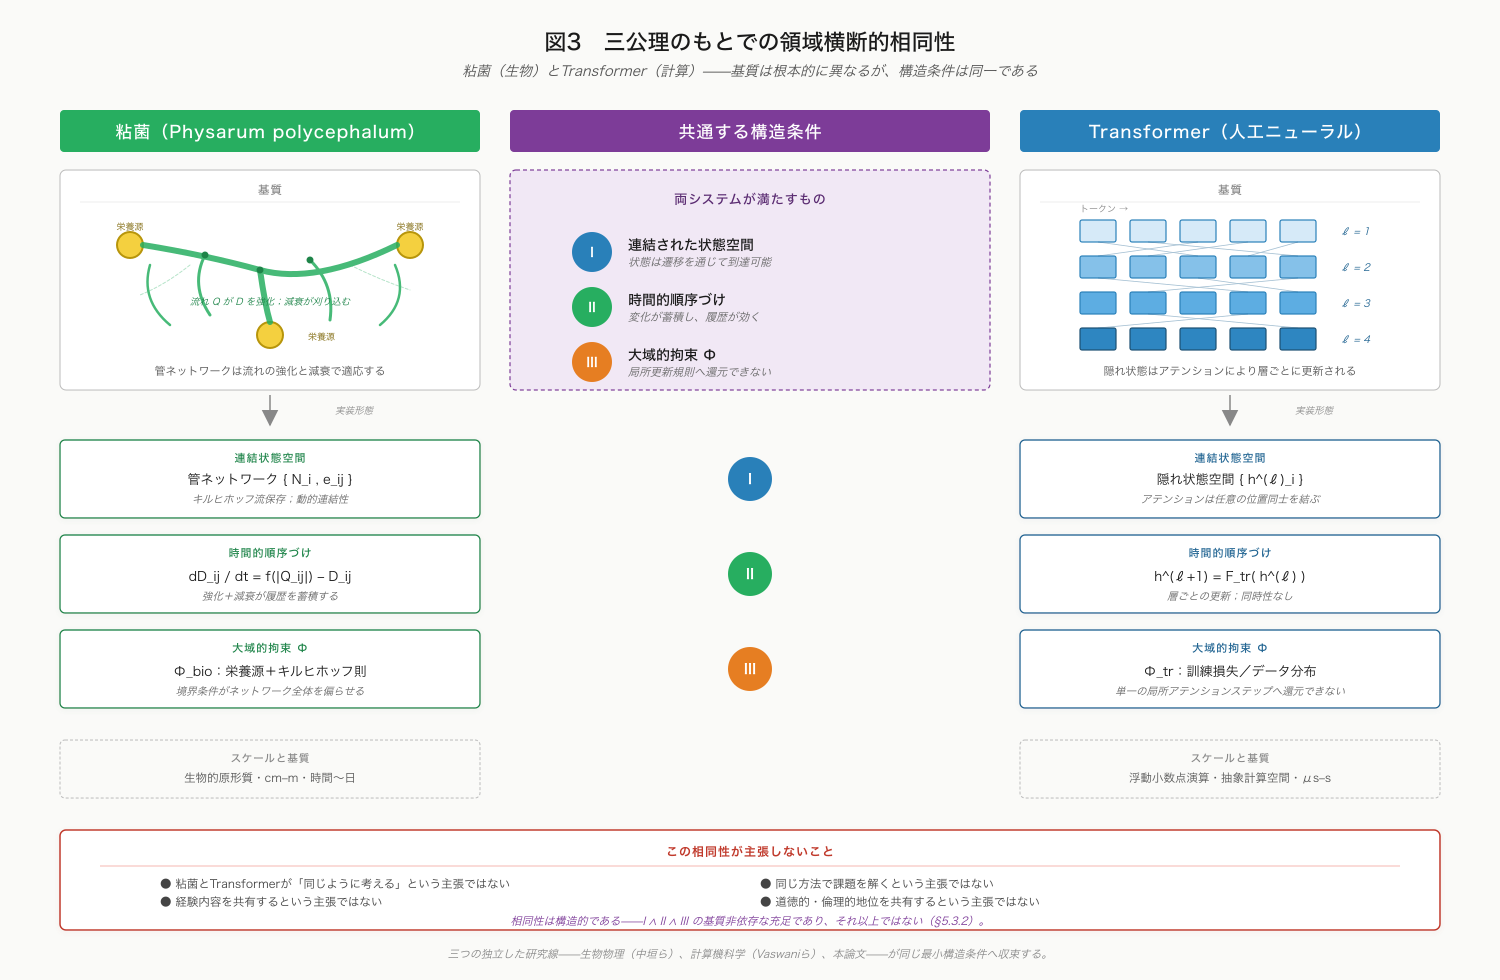
\includegraphics[width=\textwidth]{figures/fig3_cross_domain_homology_ja.png}
\caption{Cross-domain homology(粘菌の管網と Transformer の層構造を、三公理のもとで並列配置する構造図)}
\label{fig:intelligence_part1_3}
\end{figure}
